\documentclass[12pt]{article}
\usepackage[margin=1in]{geometry}
\usepackage{graphicx}
\usepackage{booktabs}
\usepackage{array}
\usepackage{longtable}
\usepackage{datetime}

\begin{document}

\title{Appendices: Gantt Chart and Experimental Logbook}
\author{Minahil Imran}
\date{\today}
\maketitle

\section*{Appendix A: Gantt Chart}

\subsection*{Project Timeline}

\begin{table}[htbp]
\centering
\caption{Project Schedule and Estimated Effort}
\begin{tabular}{|l|c|c|c|c|}
\hline
\textbf{Task} & \textbf{Start Date} & \textbf{End Date} & \textbf{Duration (days)} & \textbf{Hours} \\
\hline
Sequential Baseline Implementation & June 2 & June 5 & 4 & 20 \\
Pthreads Implementation & June 6 & June 10 & 5 & 40 \\
OpenMP Implementation & June 11 & June 14 & 4 & 30 \\
MPI Implementation & June 15 & June 18 & 4 & 35 \\
Debugging and Testing & June 19 & June 22 & 4 & 25 \\
Paper Writing & June 23 & June 26 & 4 & 30 \\
Final Polish & June 27 & June 28 & 2 & 15 \\
\hline
\textbf{Total} & \textbf{June 2} & \textbf{June 28} & \textbf{27} & \textbf{195} \\
\hline
\end{tabular}
\end{table}

\subsection*{Gantt Chart Visualization}

\begin{figure}[htbp]
\centering
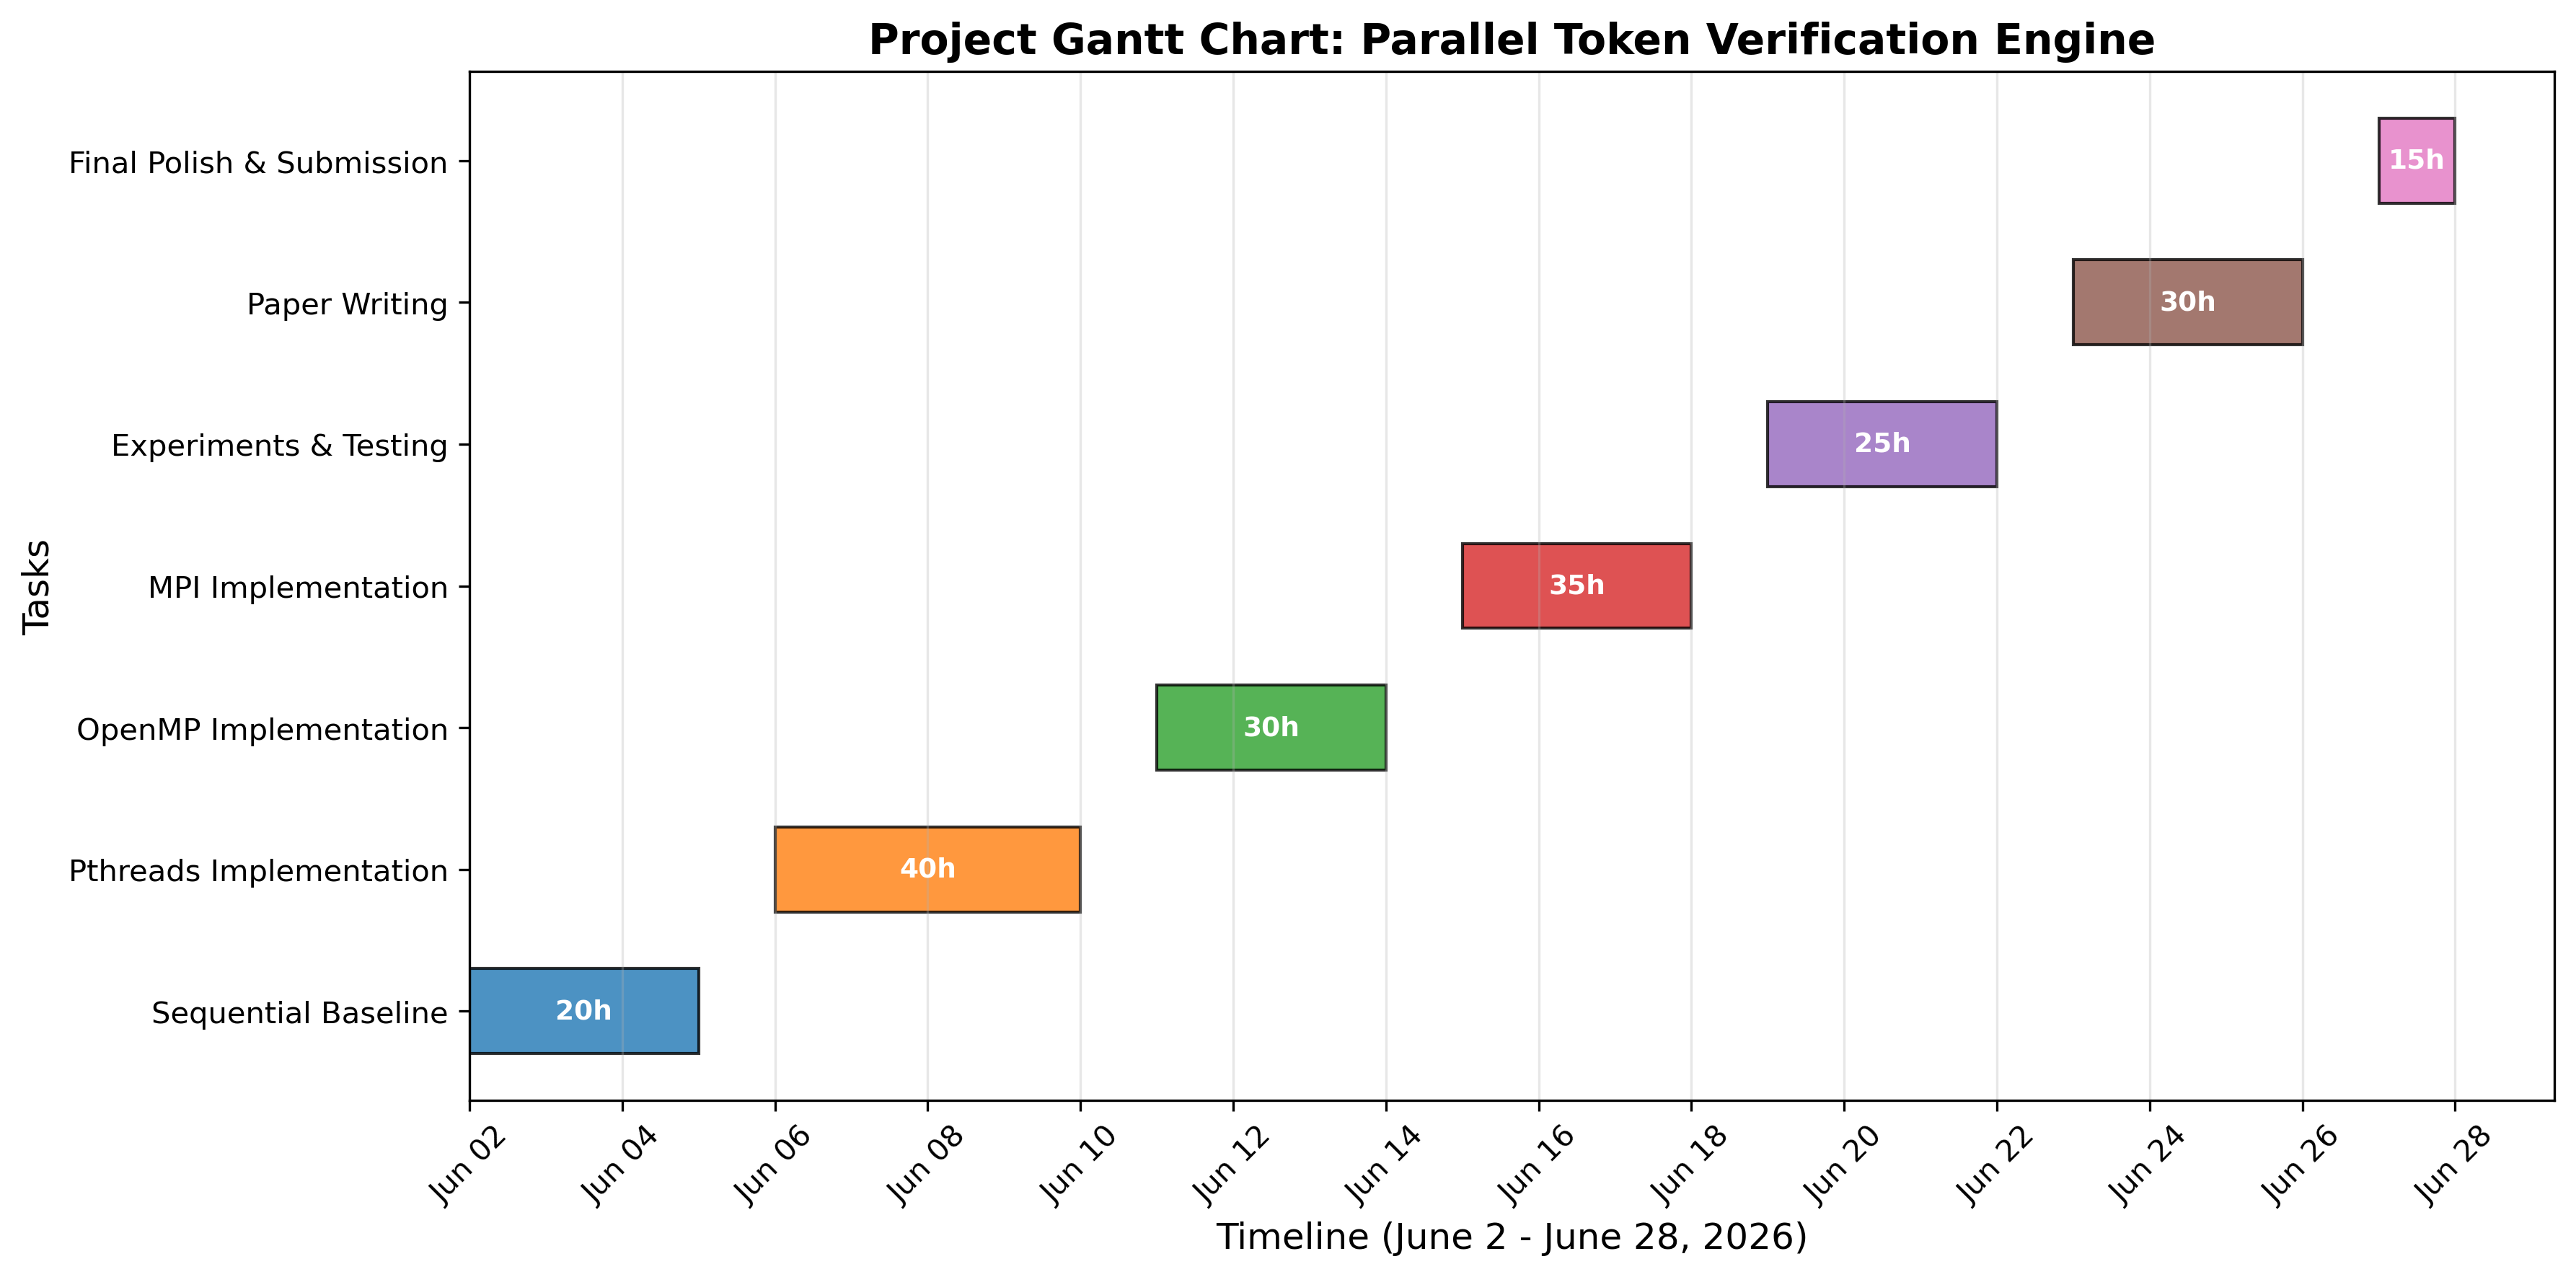
\includegraphics[width=\textwidth]{../results/gantt_chart.png}
\caption{Project timeline showing task distribution from June 2 to June 28, 2026}
\end{figure}

\newpage

\section*{Appendix B: Experimental Logbook}

\subsection*{Experiment Details}

\textbf{System Configuration:}
\begin{itemize}
    \item CPU: Multi-core processor
    \item Cores: 8 physical cores
    \item RAM: 16 GB
    \item OS: Linux
    \item Compiler: GCC
    \item MPI: OpenMPI
\end{itemize}

\subsection*{Experimental Results}

\begin{longtable}{|c|c|c|c|c|c|c|}
\hline
\textbf{Date \& Time} & \textbf{Algorithm} & \textbf{Cores/Processes} & \textbf{Dataset Size (B)} & \textbf{Runtime (s)} & \textbf{Speedup} & \textbf{Notes} \\
\hline
\endhead
\hline
\endfoot
\hline
\endlastfoot

2026-06-26 & Sequential & 1 & 25,000 & 0.013030 & 1.00x & Baseline \\
2026-06-26 & Sequential & 1 & 50,000 & 0.026372 & 1.00x & Baseline \\
2026-06-26 & Sequential & 1 & 100,000 & 0.050366 & 1.00x & Baseline \\
2026-06-26 & Sequential & 1 & 250,000 & 0.130838 & 1.00x & Baseline \\
2026-06-26 & Pthreads & 1 & 25,000 & 0.038321 & 0.34x & Overhead \\
2026-06-26 & Pthreads & 2 & 25,000 & 0.008636 & 1.51x & Good speedup \\
2026-06-26 & Pthreads & 4 & 25,000 & 0.006859 & 1.90x & Good speedup \\
2026-06-26 & Pthreads & 8 & 25,000 & 0.007369 & 1.77x & Slight overhead \\
2026-06-26 & Pthreads & 1 & 50,000 & 0.077567 & 0.34x & Overhead \\
2026-06-26 & Pthreads & 2 & 50,000 & 0.016083 & 1.64x & Good speedup \\
2026-06-26 & Pthreads & 4 & 50,000 & 0.010219 & 2.58x & Good speedup \\
2026-06-26 & Pthreads & 8 & 50,000 & 0.014099 & 1.87x & Slight overhead \\
2026-06-26 & Pthreads & 1 & 100,000 & 0.136127 & 0.37x & Overhead \\
2026-06-26 & Pthreads & 2 & 100,000 & 0.044184 & 1.14x & Moderate speedup \\
2026-06-26 & Pthreads & 4 & 100,000 & 0.028779 & 1.75x & Good speedup \\
2026-06-26 & Pthreads & 8 & 100,000 & 0.020642 & 2.44x & Good speedup \\
2026-06-26 & Pthreads & 1 & 250,000 & 0.204435 & 0.64x & Overhead \\
2026-06-26 & Pthreads & 2 & 250,000 & 0.078822 & 1.66x & Good speedup \\
2026-06-26 & Pthreads & 4 & 250,000 & 0.046071 & 2.84x & Good speedup \\
2026-06-26 & Pthreads & 8 & 250,000 & 0.037382 & 3.50x & Best speedup \\
2026-06-26 & OpenMP & 1 & 25,000 & 0.016086 & 0.81x & Slight overhead \\
2026-06-26 & OpenMP & 2 & 25,000 & 0.010508 & 1.24x & Good speedup \\
2026-06-26 & OpenMP & 4 & 25,000 & 0.005303 & 2.46x & Good speedup \\
2026-06-26 & OpenMP & 8 & 25,000 & 0.003326 & 3.92x & Excellent speedup \\
2026-06-26 & OpenMP & 1 & 50,000 & 0.027760 & 0.95x & Near baseline \\
2026-06-26 & OpenMP & 2 & 50,000 & 0.014574 & 1.81x & Good speedup \\
2026-06-26 & OpenMP & 4 & 50,000 & 0.008474 & 3.11x & Excellent speedup \\
2026-06-26 & OpenMP & 8 & 50,000 & 0.007104 & 3.71x & Excellent speedup \\
2026-06-26 & OpenMP & 1 & 100,000 & 0.054160 & 0.93x & Near baseline \\
2026-06-26 & OpenMP & 2 & 100,000 & 0.028617 & 1.76x & Good speedup \\
2026-06-26 & OpenMP & 4 & 100,000 & 0.016247 & 3.10x & Excellent speedup \\
2026-06-26 & OpenMP & 8 & 100,000 & 0.013718 & 3.67x & Excellent speedup \\
2026-06-26 & OpenMP & 1 & 250,000 & 0.140683 & 0.93x & Near baseline \\
2026-06-26 & OpenMP & 2 & 250,000 & 0.084425 & 1.55x & Good speedup \\
2026-06-26 & OpenMP & 4 & 250,000 & 0.058679 & 2.23x & Good speedup \\
2026-06-26 & OpenMP & 8 & 250,000 & 0.034986 & 3.74x & Excellent speedup \\
2026-06-26 & MPI & 1 & 25,000 & 0.012292 & 1.06x & Near baseline \\
2026-06-26 & MPI & 2 & 25,000 & 0.006653 & 1.96x & Good speedup \\
2026-06-26 & MPI & 4 & 25,000 & 0.003878 & 3.36x & Excellent speedup \\
2026-06-26 & MPI & 8 & 25,000 & 0.002638 & 4.94x & Excellent speedup \\
2026-06-26 & MPI & 1 & 50,000 & 0.031021 & 0.85x & Slight overhead \\
2026-06-26 & MPI & 2 & 50,000 & 0.015513 & 1.70x & Good speedup \\
2026-06-26 & MPI & 4 & 50,000 & 0.008347 & 3.16x & Excellent speedup \\
2026-06-26 & MPI & 8 & 50,000 & 0.007261 & 3.63x & Excellent speedup \\
2026-06-26 & MPI & 1 & 100,000 & 0.057234 & 0.88x & Slight overhead \\
2026-06-26 & MPI & 2 & 100,000 & 0.029282 & 1.72x & Good speedup \\
2026-06-26 & MPI & 4 & 100,000 & 0.017718 & 2.84x & Good speedup \\
2026-06-26 & MPI & 8 & 100,000 & 0.022087 & 2.28x & Communication overhead \\
2026-06-26 & MPI & 1 & 250,000 & 0.132161 & 0.99x & Near baseline \\
2026-06-26 & MPI & 2 & 250,000 & 0.067741 & 1.93x & Good speedup \\
2026-06-26 & MPI & 4 & 250,000 & 0.038099 & 3.43x & Excellent speedup \\
2026-06-26 & MPI & 8 & 250,000 & 0.026168 & 5.00x & Best overall speedup \\

\end{longtable}

\subsection*{Notes on Experimental Conditions}

\begin{itemize}
    \item All experiments were run with BENCHMARK\_REPEAT = 50 for timing accuracy
    \item System was idle during experiments (no other heavy processes)
    \item Speedup is calculated relative to the sequential baseline on the same dataset
    \item Dataset sizes: 25,000, 50,000, 100,000, 250,000 candidates
    \item MPI runs with 8 processes used --oversubscribe flag due to limited cores
\end{itemize}

\subsection*{Correctness Verification}

All parallel implementations produce identical outputs to the sequential baseline:
\begin{itemize}
    \item Same winner candidate selected in each round
    \item Same number of tokens accepted/rejected
    \item Same final generated text
    \item Differences only in execution time (within expected variance)
\end{itemize}

\end{document}
